\chapter{The Application}
\label{chap:application}

% ii ok o introducere asa personala?
Coming to college was the first time for me when I was on my own and I had to carefully manage my financial resources. After the first couple of months, during which I would inevitably end up short, I realized I needed a way to track my spending. I tried many methods. The first trials were using an Excel spreadsheet to record them, but that was tedious and I would often forget. Then I started looking around for other existing programs, but I didn't find any that would be acceptable. Some, like Mint \cite{mint}, that offered very detailed reports and forecasts, would get the information by linking your bank account. GnuCash \cite{gnucash}, had an extremely complicated system for doing double bookkeeping. Programs like Toshl \cite{toshl} or ExpenseIQ \cite{expenseiq} weren't doing much more than my Excel spreadsheet with a couple of charts, and entering data sure wasn't easier. 

After trying out a lot of alternatives, I decided that I would make my own program for managing my budget. It would be really easy to add expenses by taking a photo of a receipt and having OCR extract the details from the photo. There would have to be lots of reports, which can be filtered by months, shops or items, so that I could observe spending patterns and hopefully do something about them. This lead to the creation of ReceiptBudget, presented in this thesis. 

% trebuie referinte la Python, scikit-learn, Django si alte librarii?
ReceiptBudget is a web application written in Python, using the Django framework. After a user registers, he can insert expenses either manually or by taking a photo of a receipt, or he can view the dashboard of his expenses. If his expenses for the past week are over the average weekly expenses, he receives a visual warning, reminding him to be careful with what he spend his money on. 

\section{The OCR Engine}
The OCR engine does three things: it preprocesses and normalizes an image containing a receipt, it recognizes the text that is written on each line and then it extracts useful information from that text. 

For the processing of the image the OpenCV libray is used, with its Python bindings. The scikit-learn library \cite{pedregosa2011scikit} is used for the random forest and SVM implementations, while the neural networks are used from the pylearn2 library \cite{goodfellow2013pylearn2}. 
\subsection{Model design}

\subsubsection{The Random Forest Model}
The random forest was used as a model for the character segmentation problem. The criterion for choosing the best feature to split a node is the information gain (entropy). Trees are grown to their full depth, no pruning or limitation is applied to the branches. 

The other parameters of the random forest were chosen by cross-validation: the number of trees and the number of features to consider when randomly sampling from the feature space. 

\subsubsection{The Support Vector Machine Model}
The SVM was used as a baseline for the character recognition problem. The performance of both linear and radial basis function kernels was evaluated. 

The regularization parameter of the SVM was determined using cross-validation. 

\subsection{The Neural Network Model}
Neural networks were used for recognizing the characters. Various models were tried, including RBMs, Rectified Linear Units and Dropout. 


\subsection{Document Layout Analysis}
Before any characters can be recognized in a receipt, the image must first be preprocessed and normalized. This is done in several steps. 

The preprocessing consists of binarizing the images, using Otsu's method\cite{otsu1975threshold}, which adapts the threshold based on the histogram of the image. This step is done to remove any noise and speckles from the image. 

The first step in normalization is to straighten the images. The receipts are assumed to be photographed with a mobile phone camera. Users will most often take photos that are slightly rotated. The orientation of the images is assumed to be vertical, so the software will not try to identify if the receipt is horizontal. To straighten the images, they are rotated from -10 to 10 degrees, with a 0.3 angle step, and a horizontal projection (summing the pixel values row-wise) is done for each resulting image. The straight image is assumed to be the one were are the most variations between the peaks and valleys of the histogram, because in the straight image there would be high peaks because of the lines and low valleys because of the space between lines. 

The following step is removing the edges of the image, to keep only the receipt, removing any background. Due to variations in illumination, we cannot simply look for white patches to identify the receipt, because mobile cameras often use flash which gives receipts a blue tint while photos taken indoor close to a source of light have a yellow hue. The approach that was used was to look at the horizontal and vertical projections and to remove the section from the top and bottom that is over a threshold. 

The last step is detecting the lines in the receipt. Because the images are already straight and without edges, all we have to do is identify the peaks in the horizontal histogram in the image.  

The end result of the Document Layout Analysis is shown in figure \ref{fig:receipts}, where we can see a receipt that is given as an input to the engine and the output of the Document Layout Analysis, the normalized image, with the detected lines highlighted.


\begin{figure}
\centering
\begin{subfigure}{0.45\linewidth}
  \centering
  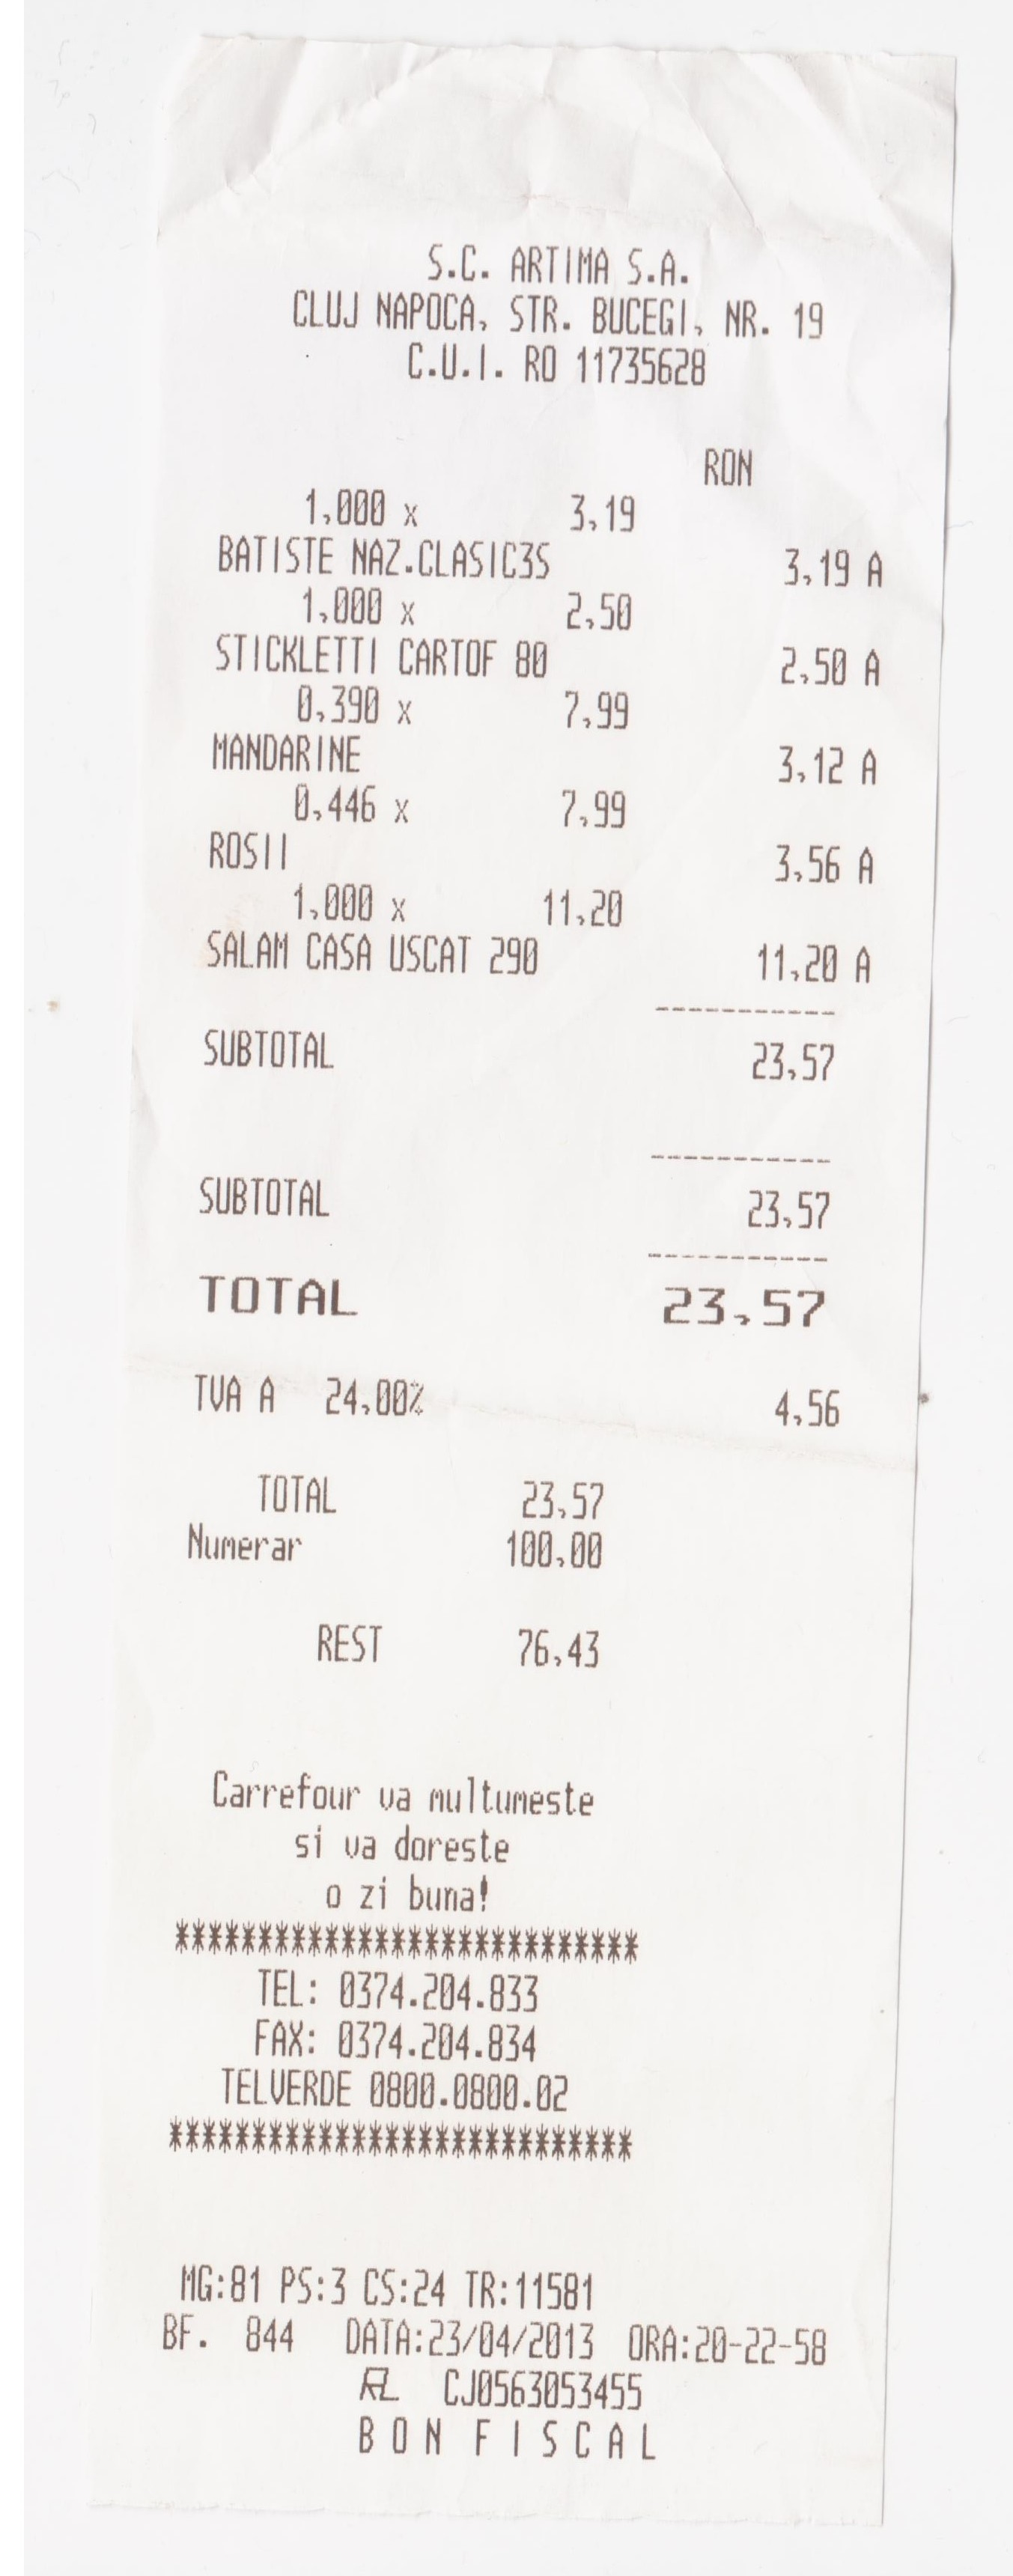
\includegraphics[width=.6\linewidth]{img/bon1.jpg}
  \caption{Example receipt}
  \label{fig:sub1}
\end{subfigure}%
\begin{subfigure}{0.45\linewidth}
  \centering
  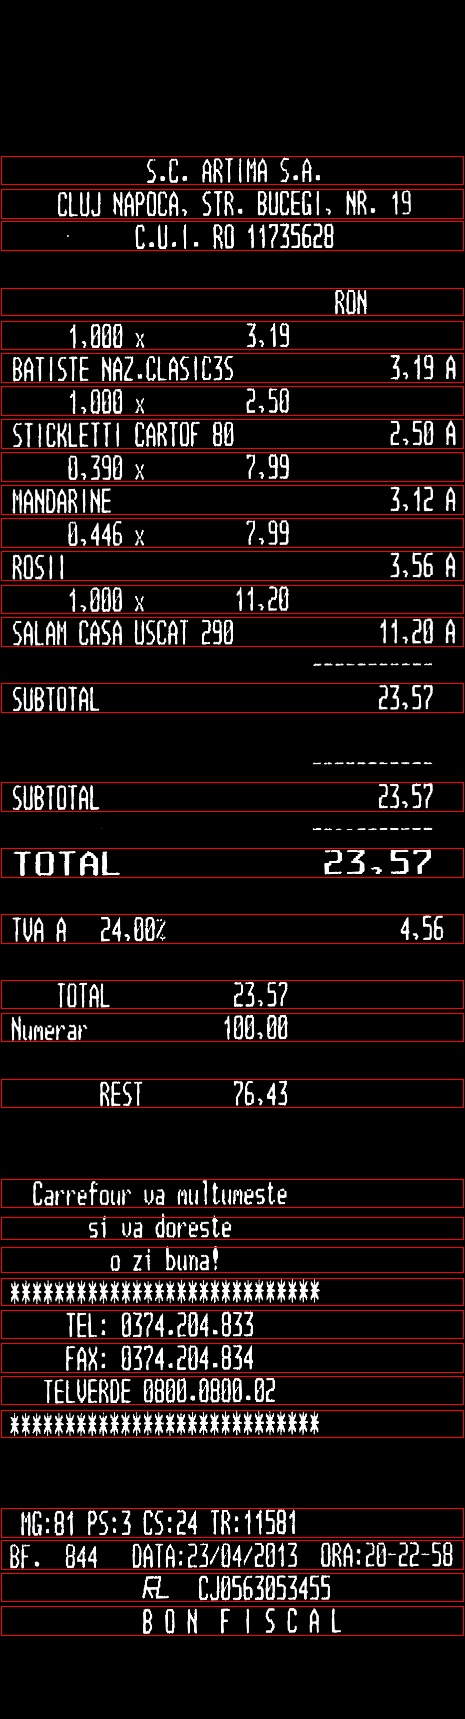
\includegraphics[width=.4\linewidth]{img/cleaned1.jpg}
  \caption{Receipt after passing through normalization}
  \label{fig:sub2}
\end{subfigure}
\caption{\label{fig:receipts}
Figure \ref{fig:sub2} is obtained after edge removal, straightening and binarization of figure \ref{fig:sub1}. Detected lines are shown with red bounding boxes.}
\label{fig:test}
\end{figure}


\subsection{Experimental Evaluation}
In this section we describe the experiments that we have done, starting with the data gathering process, the training of the models and the results of their evaluation.

\subsection{Data Set and Processing}
The data set was obtained from 20 receipts that were manually annotated with the position of each character in them. In total there are 7045 characters. There are 74 different characters, including digits, uppercase and lowercase letters and punctuation. 

The bounding boxes of the characters were extracted from the images. The resulting patches were normalized to have a size of 30x30 pixels and were converted to grayscale. The small images that resulted after this processing were used as the data set for the character recognition problem.

For the character segmentation problem, positive and negative patches were extracted from the images, each containing 40 columns of pixels. The positive example were obtained by taking the leftmost and rightmost columns of the bounding boxes of characters, together with 19 previous columns and 20 columns that followed. The negative examples were obtained by sampling randomly from the middle of a character and taking 19 columns from before and 20 from after.

For the character recognition problem, the labels corresponding to each character were converted to a vector of 74 dimensions, with each dimension corresponding to one possible character value. The value of the dimension corresponding to the character of a data point was set to 1, while all the others were set to 0. 

For the character segmentation problem, the labels were binary: 1 if a certain data point was were a segmentation should occur, 0 otherwise. 

\subsection{Training and Testing}
The data set was shuffled and then split into two parts, one for training and one for testing. The splitting was done in a random way, because the data points are independent and order does not matter. The training set contained 80\% of the data and the test set contained the remaining 20\%. 

All experiments were run multiple types, with the dataset being shuffled each time. In the case of the Random Forests, the multiple runs of the experiments are necessary because the splitting points for the trees and the dataset splits are chosen randomly across runs. In the case of the neural networks, the initialization of the weights between neurons was random. 
\subsection{Results}
\label{sec:recog}
For both tasks, the parameters for the algorithms were selected using cross-validation. In the case of the SVM, the search space was on logarithmic scale from $10^{-2}$ to $10^4$ for the regularization parameter. In the case of the random forest, the number of trees used ranged from 150 to 250, in steps of 50, and the number of features to be sampled at each point varied from using the square root, the base 2 logarithm, 10\% or 30\% of the total number of features. For the neural network, there was an experiment where a RBM was used for unsupervised pretraining which then was used to initialize an MLP with 2 hidden layers. The parameters in this case were the learning rate which varied from 0.01 to 0.5 and the number of neurons in 10 increments, which ranged from 200 to 1000 in steps of 100. The other neural network setup was a four layered MLP, where each layer was with ReLU and dropout was applied to the layers. In this case the parameters that varied were the learning rate, the momentum and the number of neurons for each layer. 

Table \ref{table:recog_values} contains the average, maximum and minimum values obtained for the accuracy of the character recognition problem.

% Please add the following required packages to your document preamble:
% \usepackage{booktabs}
\begin{table}[h]
\caption{The accuracy for the character recognition experiment}
\label{table:recog_values}
\begin{tabular}{llllll}
\hline
Kernel type & Regularization & Min     & Max     & Mean    & Std. dev. \\ \hline
RBF & 0.01 & 0.09141 & 0.09207 & 0.09165 & 0.00030 \\ 
Linear & 0.01 & 0.71585 & 0.71768 & 0.71672 & 0.00075 \\ 
RBF & 1 & 0.59146 & 0.60671 & 0.60130 & 0.00697 \\ 
Linear & 1 & 0.90372 & 0.90610 & 0.90490 & 0.00097 \\ 
RBF & 100 & 0.90854 & 0.91159 & 0.91018 & 0.00126 \\ 
Linear & 100 & 0.89695 & 0.90006 & 0.89860 & 0.00128 \\ 
RBF & 1000 & 0.90183 & 0.91341 & 0.90795 & 0.00475 \\ 
Linear & 1000 & 0.89207 & 0.89762 & 0.89453 & 0.00231 \\ 
RBF & 10000 & 0.90671 & 0.91220 & 0.90957 & 0.00225 \\ 
Linear & 10000 & 0.89146 & 0.89762 & 0.89494 & 0.00258 \\ \hline
\end{tabular}
\end{table}

In this case, using RBF kernel SVM resulted in a $ 91.018\% \pm 0.126 $ accuracy in the best case, using a value of 100 for the regularization rate, while using a linear kernel yielded $ 90.490\% \pm 0.097 $ as its best result, for the value of 1 for the regularization rate. A RBF kernel gives a slightly better results.

Figure \ref{fig:conf_matrix} contains the confusion matrix for the best experiment on the character recognition problem.



\begin{figure}[h!]
\begin{center}
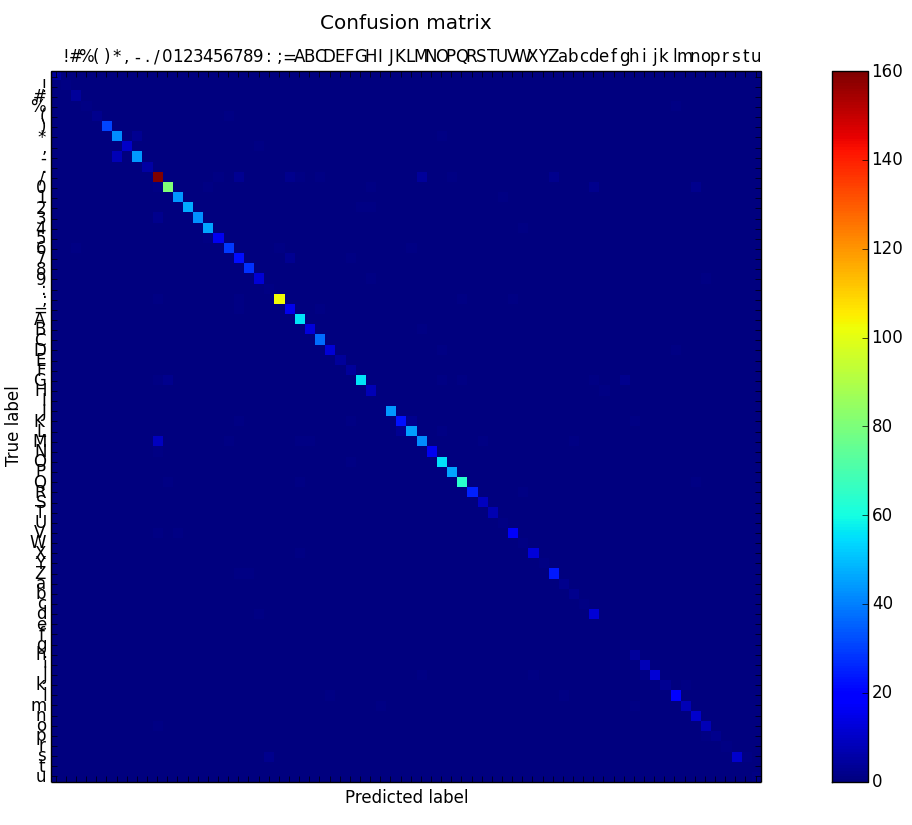
\includegraphics[width=0.8\linewidth]{img/rec_cm.png}
\caption{\label{fig:conf_matrix}
Confusion matrix for the best model for the character recognition problem}
\end{center}
\end{figure}

Table \ref{table:seg_values} contains the average, maximum and minimum values obtained for the F1 measure\cite{fawcett2006introduction} of the character segmentation problem. The F1 measure is used instead of the accuracy because the two classes are imbalanced: there are 11475 data points which indicate a segmentation point, while there are 19402 points which are not segmentation points, almost twice as many. 

\begin{table}[h]
\caption{The F1 score for the character segmentation experiment}
\label{table:seg_values}
\begin{tabular}{llllll}
\hline
Nr. trees & Nr. features & Min     & Max     & Mean    & Std. dev. \\ \hline
150 & 20 & 0.87318 & 0.88326 & 0.87735 & 0.00363 \\ 
200 & 20 & 0.86975 & 0.88312 & 0.87657 & 0.00490 \\ 
250 & 20 & 0.87258 & 0.88776 & 0.87773 & 0.00531 \\ 
150 & 8 & 0.86894 & 0.88376 & 0.87569 & 0.00517 \\ 
200 & 8 & 0.87227 & 0.88299 & 0.87675 & 0.00413 \\ 
250 & 8 & 0.87178 & 0.88470 & 0.87717 & 0.00426 \\ 
150 & 120 & 0.87262 & 0.88631 & 0.87816 & 0.00476 \\ 
200 & 120 & 0.87122 & 0.88387 & 0.87724 & 0.00418 \\ 
250 & 120 & 0.87367 & 0.88565 & 0.87885 & 0.00391 \\ 
150 & 40 & 0.87073 & 0.88671 & 0.87822 & 0.00552 \\ 
200 & 40 & 0.86980 & 0.88519 & 0.87845 & 0.00513 \\ 
250 & 40 & 0.87358 & 0.88671 & 0.87936 & 0.00445 \\  \hline
\end{tabular}
\end{table}

The confusion matrix for the best experiment on the character segmentation problem is presented in table \ref{table:seg_conf}.

\begin{table}[h]
\caption{The confusion matrix for the character segmentation experiment}
\label{table:seg_conf}
\begin{tabular}{lll}
\hline
 & No split & Split \\ \hline
Predicted no split & 4556 & 363 \\ 
Predicted split & 255 & 2546 \\  \hline
\end{tabular}
\end{table}
\section{Development}
\subsection{Requirements Analysis}
\subsection{Designing}
\subsection{Implementation}
\section{User Manual}
\label{sec:manual}
\section{Discussion}